\Testart{Skript}
\Klasse{09}
\Fach{Informatik}
\Titel{Tabellenkalkulation}
\Lehrer{Valentin Herrmann}

    
%\large

\renewcommand{\Content}{

    \mysession{Stunde 1+2}{
    
        \Aufgabe{BYCS Drive}{%
    \begin{minipage}[t]{0.5\textwidth}
        \vspace{0pt}
        \begin{enumerate}
            \item Öffne \UrlAndCode{drive.bycs.de} im Internetbrowser und melde dich mit deinen BYCS/Mebis Logindaten an. \\
                \hinweis{Internetbrwoser zeigen Websites an und sind unser üblicher Zugang zum Internet. Bekannte Browser sind \textbf{Mozilla Firefox}, Google Chrome oder Microsoft Edge.}
            \item Erstelle einen in deinem persönlichen Bereich einen neuen Ordner mit Name \emph{Informatik\_09}
            \item Wenn du in diesem Ordner auf \emph{+Neu} klickst kannst du neue Dateien (z.B. Kalkulationstabellen) erstellen.\\
                \emphColB{WICHTIG:} Achte darauf, die Dateiendung (nach dem Punkt, z.B. \emphColB{.xlsx}), nicht zu verändern!
        \end{enumerate}
    \end{minipage}
    \hfill
    \begin{minipage}[t]{0.45\textwidth}
        \ifbeamer
            \vspace{3.5cm}
        \else
            \vspace{0pt}
        \fi
        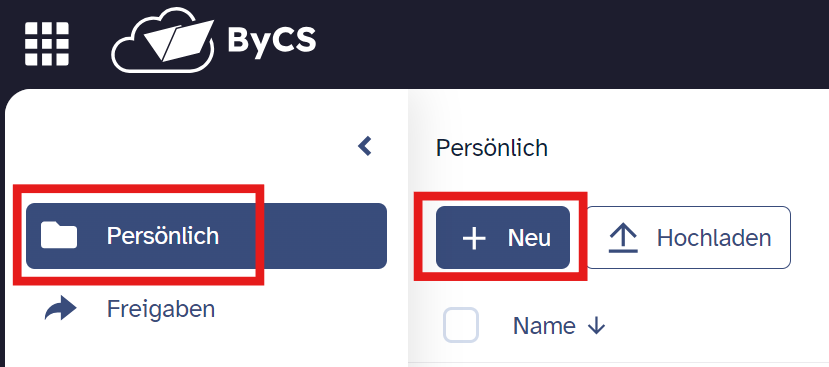
\includegraphics[width=\textwidth]{_Aufgaben/img/A00_newFolder.png}
    \end{minipage}
}

        
        \Aufgabe[30]{Excel Werbung}{ 
    \begin{enumerate}
      \item Schau das Video unter: \UrlAndCode{mebis.link/inf9\_excel-werbung}
      \item Erstelle in BYCS-Drive eine neue Kalkulationstabelle \emphColB{01\_ExcelWerbung.xlsx}\\
        \hinweis{Es gibt verschiedene Systeme zur Wahl von Dateinamen. Hier ist einem Nummerierung am Anfang gewählt; möglich wäre auch ein Datum am Anfang (z.B. 2025-09-25\_ExcelWerbung.xlsx)}
      \item Baue die Tabelle aus dem Video mit den exakt gleichen Schritten in BYCS-Drive nach!
      \item Füge deiner Tabelle ein Diagramm hinzu, das die Quartalszahlen grafisch darstellt.
      \item Stellt die Tabelle tatsächlich eine Wachstumsrate von 10\% von Quartal zu Quartal dar?\\
        \hinweis{10\% von 1000€ sind etwas anderes als 10\% von 1100€}
      \item Falls nein, wie könnte man die Einträge so ändern, dass automatisch 10\% Wachstumsrate berechnet werden?
    \end{enumerate}

    \AttachLsg{\faFileExcelO}{_Aufgaben/resources/A01_Lsg.xlsx}
}
        
        \Hefteintrag{1.8}{Tabellenkalkulation}{ In Tabellenkalkulationsprogrammen können Daten in den Zellen der \LoesungLuecke{Tabellenblätter}{6cm} erfasst und mithilfe von \emphColA{Formeln} verarbeitet werden. Jede Zelle besitzt eine eindeutige \emphColA{Adresse}. Diese besteht aus \emphColA{Buchstaben (\LoesungLuecke{Spalten}{4cm}) und Zahlen (\LoesungLuecke{Zeilen}{4cm})}.
%
Bekannte Tabellenkalkulationsprogramme sind z.B. Microsoft Excel, LibreOffice Calc oder Google Spreadsheets. }
    }
    
    \mysession{Stunde 3+4}{
    
        \Hefteintrag{2}{Formeln und Parameter}{
    \doppelseite{0.44}{0.53}{t}{%
        \LoesungLuecke{Formeln}{6cm} berechnen Zellwerte automatisch. Sie beginnen immer mit einem \LoesungLuecke{Gleichheitszeichen (=)}{8cm} gefolgt von einem mathematischen Term oder vorgefertigten Funktionen (z.B. Mittelwert). Die \emphColA{Grundrechenarten} werden dargestellt als: \emphColA{\LoesungLuecke{+}{0.5cm} , \LoesungLuecke{-}{0.5cm} , \LoesungLuecke{*}{0.5cm} , \LoesungLuecke{/}{0.5cm}}
        
        In Formeln können feste Werte (z.B. für MwSt: 1,19) oder Werte anderer Zellen (als Adresse, z.B. B5) als Parameter verwendet werden. Die Berechnung des Ergebnisses nennt man auch Auswertung der Formel und läuft so ab:
    }
    {
        \LoesungKaroTikz{
            \pause\pause\pause\pause\pause\pause\pause
            \node[box] (formula) {Formel};
            \pause
            \node[annotation, below left=0.2cm and -2.5cm of formula] (fexample) {z.B. =1,19*B5};
            \pause
            \node[box, rounded corners=1pt, right=2.5cm of formula] (cellvalues) {Zellwerte};
            \pause
            \node[annotation, below right=0.2cm and -2.3cm of cellvalues] (cexample) {z.B. 100};
            \pause
            \node[box, rounded corners=1pt, below=7cm of $(formula)!0.5!(cellvalues)$] (final) {Endergebnis};
            \pause
            \node[annotation, above right=0.1cm and -1.4cm of final] (fexample) {z.B. 119};
            \pause 
            \node[oval, text width=5cm, below=1.5cm of $(formula)!0.5!(cellvalues)$] (replace) {Adressen durch Zellwerte ersetzen};
            \draw[arrow] (formula) -- (replace);
            \draw[arrow] (cellvalues) -- (replace);
            \pause
            \node[annotation, below right=0.5cm and -2.5cm of replace] (rexample) {z.B. = 1,19*100};
            \pause
            \node[oval, below=1cm of replace] (calc) {Ergebnis berechnen};
            \draw[arrow] (replace) -- (calc);
            \pause
            \draw[arrow] (calc) -- (final);
        }{25}
    }
}
        
        \Aufgabe[25]{Excel-Werbung erweitert mit Formeln}{
    %\AttachVlgLsg{\faFileExcelO}{_Aufgaben/resources/A01_Lsg.xlsx}{_Aufgaben/resources/A02_Lsg.xlsx} 
    \doppelseite{0.56}{0.4}{t}{
        \begin{enumerate}
            \item Öffne deine Excel-Datei von letzter Stunde und lege mit dem + am unteren Rand ein neues Tabellenblatt an.
            \item Führt die Schritte wie im Video aus, jedoch nur bis zu den Werten der 1. Spalte
            \item Vervollständigt die Tabelle so, dass die Wachstumsrate (bisher 10\%) in einer eigenen Zelle gespeichert und von euren Formeln verwendet wird.
            \item Überlegt euch ein System, um die Art der Zelle optisch hervorzuheben und setzt dies in eurer Tabelle um. Tragt hierfür zunächst jede Art in eine eigene Zelle ein und hebt auch diese Zellen entsprechend hervor. Die Tabelle hat diese Zellarten: \emphColA{Beschriftung}, \emphColB{Eingabewert}, \emphColC{automatische Berechnung (=Formel)}
        \end{enumerate}
    }{
        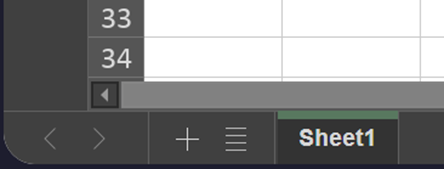
\includegraphics[width=\textwidth]{_Aufgaben/img/A02_newSheet.png}
    }
}

        
        \Hefteintrag{1.5}{Absolute und relative Zellbezüge}{
\doppelseite{0.44}{0.54}{t}{
Zieht oder kopiert man eine Formel in eine andere Zelle, so verändern sich die Adressen entsprechend der veränderten Zellposition. Man spricht von einem  \emphColA{\LoesungLuecke{relativen}{5cm} Zellbezug}.

Möchte man dies verhindern, setzt man ein \emphColB{\$-Symbol} vor den entsprechenden Teil (Zeile oder Spalte) der Adresse und spricht von einem \emphColB{\LoesungLuecke{absoluten}{5cm} Zellbezug}. Dies ist auch für Spalte oder Zeile einzeln möglich.
}{
\centering
\emphColB{Beispiel:}

\vspace{0.1cm}
\begin{tabular}{c|c|c}
    \makecell{Art des \\ Bezugs von A1} & 
    \makecell{Original\\Formel} 
    & \makecell{2 nach unten \\ + 1 nach rechts\\verschoben}\\
    \hline\hline
    relativ & 
    = A1 + C3 &
    \LoesungLeer{=B3 + D5}{0pt}\\
    \hline
    \makecell{Spalte absolut\\Zeile relativ} &
    = \$A1 + C3 & 
    \LoesungLeer{=\$A3 + D5}{0pt}\\
    \hline
    \makecell{Spalte relativ\\Zeile absolut} & 
    = A\$1 + C3 & 
    \LoesungLeer{=B\$1 + D5}{0pt}\\
    \hline
    absolut & 
    = \$A\$1 + C3 & 
    \LoesungLeer{=\$A\$1 + D5}{0pt}\\
\end{tabular}
}
}

    }
    
    \mysession{Stunde 5+6}{

        \Aufgabe[15]{Formeln mit Diagrammen darstellen}
{
Diagramme wie im ersten Hefteintrag, die Eingabe, Verarbeitung und Ausgabe darstellen, nennt man Datenflussdiagramm.
\begin{itemize}
    \item Zeichne für eine Wachstumsberechnung und eine Summe aus deiner Tabelle je ein Datenflussdiagramm.
    \item Überlege dabei: Wie stellst du die Daten dar und wieso?\\Zum Beispiel als konkreten Wert, als Zelladresse, als Beschreibung, ... ?
\end{itemize}
\LoesungKaroTikz{
    \node[box, text width=2cm] (gq2) {Umsatz Golf Q2};
    \node[box, text width=2.1cm, right=0.3cm of gq2] (tq2) {Umsatz Tennis Q2};
    \node[box, text width=2.1cm, right=0.3cm of tq2] (sq2) {Umsatz Safari Q2};

    \node[oval, text width=2.2cm, below=1cm of tq2] (summe) {SUMME (nicht + ! )};
    
    \node[box, below=1cm of summe] (final) {Gesamtumsatz Q2};
    
    \draw[arrow] (gq2) -- (summe);
    \draw[arrow] (tq2) -- (summe);
    \draw[arrow] (sq2) -- (summe);
    \draw[arrow] (summe) -- (final);
    %
    %
    %
    \node[box, text width=2.1cm, right=1cm of sq2] (golf) {Umsatz Golf Q2};
    \node[box, text width=2.1cm, right=0.3cm of golf] (fakt) {Wachstums-faktor};

    \node[oval, text width=2.2cm, below=1cm of $(golf)!0.5!(fakt)$] (stern) {PRODUKT oder *};
    
    \node[box, below=1cm of stern] (gq3) {Umsatz Golf Q3};
    
    \draw[arrow] (golf) -- (stern);
    \draw[arrow] (fakt) -- (stern);
    \draw[arrow] (stern) -- (gq3);
}{22}
}
    
        \Hefteintrag{2}{Exkurs: Abstraktionsebenen}{

Ein Kerngebiet der Informatik ist es, Programme darzustellen. Die Arbeit eines Computers ist sehr komplex, daher nutzt man \LoesungLuecke{Abstraktion (Trennung von Konzept und Umsetzung)}{11cm}.



%\emphColA{Abstraktion (=Trennung von Konzept \& konkreter Umsetzung)}.
Je nach Anwendung ist ein anderer Detailgrad notwendig. Man spricht dann von verschiedenen \LoesungLuecke{Abstraktionsebenen}{10cm}. In einem Modell (\LoesungLuecke{= Abbild der Realität, z.B. als Diagramm}{15cm}) stellt man alles möglichst auf derselben Ebene dar. 

\vspace{1cm}

Mögliche Abstraktionsebenen einer Zelle unserer Tabelle (es gibt mehr!):

\centering
\vspace{0.5cm}
\large
\begin{tabular}{c|c|c|c}
    tatsächlicher Wert & Formel m. Adresse & Beschreibung Einzelwerte & Beschreibung   \\\hline
    \Loesung{3630€}& \Loesung{=E5 * \$C\$3} & \Loesung{=GolfQ2 * Wachstumsfak.} & \Loesung{Umsatz Golf Q3} \\ 
\end{tabular}
}
        
        \Aufgabe{Der Weg der Daten}{
    \begin{minipage}[t]{0.85\textwidth}
        \begin{enumerate}
            \item Öffne im Browser Orinoco: \UrlAndCode{klassenkarte.de/oo/} 
            \item Aus der linken Spalte benötigen wir die Elemente \emphColB{Eingabe, Funktion, Ausgabe und Datenfluss}.
            \item Wähle zwei verschiedene Formelfelder deiner Tabelle aus und erstelle ein Diagramm mit den genannten Elementen, das darstellt, welche Daten in die Berechnung einfließen, welche ausgegeben werden und was für eine Berechnung durchgeführt wird. 
            \item Erstellt möglichst viele Diagramme auf verschiedenen Abstraktionsebenen.
        \end{enumerate}
        
        \vspace{0.2cm}
        \Loesung{
            Ein paar Beispiele für eine Zelle. Es gibt natürlich seehr viele   Möglichkeiten.\\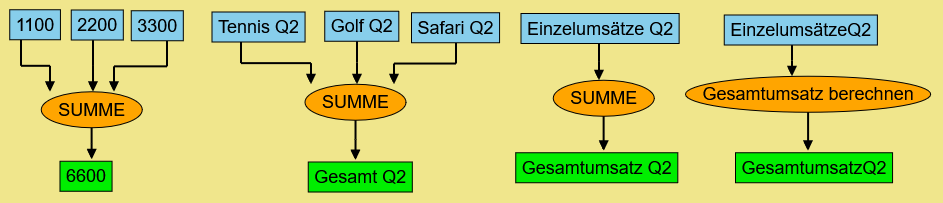
\includegraphics[width=\textwidth]{_Aufgaben/img/orinoo.png}
        }
    \end{minipage}
}
    }
    
    \mysession{Stunde 7+8}{
        
        \Hefteintrag{1}{Datenflussdiagramm}{
    \doppelseite{0.47}{0.47}{t}{
        Datenflussdiagramme stellen die \emphColA{Ein- und Ausgaben von Funktionen} übersichtlich dar. Man nutzt sie, um die Umsetzung eines Programms zu \emphColA{planen oder} im Nachhinein zu \emphColA{dokumentieren}. Datenflussdiagramme bestehen aus diesen Elementen:

        \vspace{0.3cm}
        \LoesungKaroTikz{
                \node[box, rounded corners=1pt, text width=4cm, minimum width=1pt] (werte) {Werte (Eingaben/Ausgaben)};

                \node[oval, text width=2.2cm, right=0.2cm of werte] (fkt) {Funktionen};
                
                \node[minimum width=1pt, below=1cm of werte] (d1) {Datenflüsse: };
                \node[minimum width=1pt, right=1cm of d1] (d2) { };
                \draw[arrow] (d1)--(d2);
        }{16}
    }{
        \emphColA{Schema eines DFDs mit Platzhaltern:}

        \vspace{0.2cm}
        \LoesungKaroTikz{
            \node[box, rounded corners=1pt, text width=1.7cm, minimum width=1pt] (e1) {Eingabe 1};
            \node[box, rounded corners=1pt, text width=0.5cm, minimum width=1pt, minimum height=8pt, right=0.2cm of e1] (e2) {...};
            \node[text width=0.5cm, minimum width=1pt, minimum height=8pt, right=0.2cm of e2] (edots) {...};
            \node[box, rounded corners=1pt, text width=0.5cm, minimum width=1pt, minimum height=8pt, right=0.2cm of edots] (e3) {...};
            \node[box, rounded corners=1pt, text width=1.7cm, minimum width=1pt, right=0.2cm of e3] (eN) {Eingabe n};

            \node[oval, text width=2.2cm, below=1cm of edots] (fkt) {Funktion};
            
            \node[box, rounded corners=1pt, below=1cm of fkt] (final) {Ausgabe (genau eine!)};
            
            \draw[arrow] (e1) -- (fkt);
            \draw[arrow] (e2) -- (fkt);
            \draw[arrow] (e3) -- (fkt);
            \draw[arrow] (eN) -- (fkt);
            \draw[arrow] (fkt) -- (final);
        }{22}
    }
}

    
        \Hefteintrag{2}{Funktionen und Stelligkeit}{
Eine Funktion besitzt in der Informatik genauso wie in Mathe Eingaben (=\LoesungLuecke{Parameter}{4.7cm}) und genau eine Ausgabe (=\LoesungLuecke{Rückgabewert}{6cm}).

Besitzt eine Funktion \emphColA{einen} Parameter heißt sie \LoesungLuecke{einstellig}{6cm}, bei \emphColA{zwei} Parametern \LoesungLuecke{zweistellig}{6cm} usw.

Gewöhnliche \emphColA{Rechenoperationen sind \LoesungLuecke{zweistellige}{6cm} Funktionen}. SUMME und PRODUKT können auch als fertige Funktion geschrieben werden und sind dann \emphColB{beliebig vielstellig}. 

Einzelne \emphColA{Parameter trennt} man mit \emphColA{Semikolon}, alle Zellen innerhalb eines \emphColB{Bereichs} gibt man mit \emphColB{Doppelpunkt zwischen Start- und Endzelle} an. \emphColA{Zum Beispiel:}

\vspace{0.3cm}
\LoesungLuecke{= A1 + B1 + C1 + D1 = SUMME(A1;B1;C1;D1) = SUMME(A1:D1)}{17.5cm}
}
        
        \Aufgabe{Getränkekalkulation}
{
    \AttachVlg{\faFilePdfO}{_Aufgaben/resources/A05_Stationen.pdf}
    Ihr macht die Kalkulation für eine große Party mit einer Kalkulationstabelle. Da so eine Planung aufwendig ist, wird sie auf mehrere Personen aufgeteilt.
    \begin{enumerate}
        \item Bildet mindestens 4 Gruppen (A1,A2,B1,B2 - manche kann es doppelt geben) und nehmt euch gemeinsam einen Zettel. Eure Aufgabenstellung erhaltet ihr von der Lehrkraft \Loesung{(oben als Dateianhang)}
        \item Zeichnet zu eurer Aufgabenstellung \emphColB{pro Schritt ein Datenflussdiagramm} (mit hoher Abstraktion)\\
            \hinweis{Hohe Abstraktion bedeutet keine konkreten Rechnungen, sondern beschreibende Funktionsnamen.}\\
            \hinweis{Wenn die gleiche Berechnung für mehrere Getränke gemacht wird, zeichnet hierfür mehrere Diagramme.}
        \item Tauscht euer Diagramm mit der anderen Gruppe eures Buchstabens (also z.B. tauschen A1 und A2) und setzt dieses dann mit der Tabellensoftware in BYCS-Drive um. \begin{itemize}
        \item Färbt auch dieses Mal wieder die Zellen anhand des Typs (Nutzereingabe, Formel, Beschriftung) ein.
            \item Zum Testen eurer Formeln könnt ihr einfach Preise und Gäste-Anzahlen erfinden.
            %\item Beantwortet außerdem folgende Fragen:
        \end{itemize}
    \end{enumerate}

    Wieso ist es sinnvoll, zuerst ein Diagramm zu zeichnen?

    \LoesungLine{z.B. Besserer Überblick, Aufbau einer Intuition für den Kontext, geringere Gefahr vor lauter Syntax den Überblick zu verlieren, 'Divide-and-Conquer', erst Planen, dann Umsetzen reduziert Fehler}{2}


    Welche Eigenschaften eines Diagramms machen die Umsetzung leichter?

    \LoesungLine{aussagekräftige Namen für Werte auch ohne den Kontext zu kennen, beschreibende Funktionsnamen statt nur Rechenoperationen, \dots}{2}
}
\UnterAufgabe{Getränkekalkuation A1}{

    \ifbeamer\else
    \Loesung{\textbf{Gruppe A1}}
    \fi
    
    \LoesungTikz{
            \node[dfddata, text width=2cm, minimum width=1pt] (e1) {Preis Kasten Spezi};
           % \node[dfddata, text width=0.5cm, minimum height=8pt, right=0.2cm of e1] (e2) {...};
            %\node[text width=0.5cm, minimum width=1pt, minimum height=8pt, right=0.2cm of e2] (edots) {...};
            %\node[dfddata, text width=0.5cm, minimum height=8pt, right=0.2cm of edots] (e3) {...};
            \node[dfddata, text width=3cm, right=0.2cm of e1] (eN) {Anzahl Flaschen pro Kasten Spezi};

            \node[oval, text width=3.5cm, below=1.5cm of $(e1)!0.5!(eN)$] (fkt) {Flaschenpreis Spezi berechnen};
            
            \node[dfddata, below=0.5cm of fkt] (final) {Flaschenpreis Spezi};
            
            \draw[arrow] (e1) -- (fkt);
            %\draw[arrow] (e2) -- (fkt);
            %\draw[arrow] (e3) -- (fkt);
            \draw[arrow] (eN) -- (fkt);
            \draw[arrow] (fkt) -- (final);
    }
    \LoesungTikz{
            \node[dfddata, text width=2cm, minimum width=1pt] (e1) {Preis Kasten Wasser};
           % \node[dfddata, text width=0.5cm, minimum height=8pt, right=0.2cm of e1] (e2) {...};
            %\node[text width=0.5cm, minimum width=1pt, minimum height=8pt, right=0.2cm of e2] (edots) {...};
            %\node[dfddata, text width=0.5cm, minimum height=8pt, right=0.2cm of edots] (e3) {...};
            \node[dfddata, text width=3cm, right=0.2cm of e1] (eN) {Anzahl Flaschen pro Kasten Wasser};

            \node[oval, text width=3.5cm, below=1.5cm of $(e1)!0.5!(eN)$] (fkt) {Flaschenpreis Wasser berechnen};
            
            \node[dfddata, below=0.5cm of fkt] (final) {Flaschenpreis Wasser};
            
            \draw[arrow] (e1) -- (fkt);
            %\draw[arrow] (e2) -- (fkt);
            %\draw[arrow] (e3) -- (fkt);
            \draw[arrow] (eN) -- (fkt);
            \draw[arrow] (fkt) -- (final);
    }
    \LoesungTikz{
            \node[dfddata, text width=2cm, minimum width=1pt] (e1) {Preis Kasten Bier};
           % \node[dfddata, text width=0.5cm, minimum height=8pt, right=0.2cm of e1] (e2) {...};
            %\node[text width=0.5cm, minimum width=1pt, minimum height=8pt, right=0.2cm of e2] (edots) {...};
            %\node[dfddata, text width=0.5cm, minimum height=8pt, right=0.2cm of edots] (e3) {...};
            \node[dfddata, text width=3cm, right=0.2cm of e1] (eN) {Anzahl Flaschen pro Kasten Bier};

            \node[oval, text width=3.5cm, below=1.5cm of $(e1)!0.5!(eN)$] (fkt) {Flaschenpreis Bier berechnen};
            
            \node[dfddata, below=0.5cm of fkt] (final) {Flaschenpreis Bier};
            
            \draw[arrow] (e1) -- (fkt);
            %\draw[arrow] (e2) -- (fkt);
            %\draw[arrow] (e3) -- (fkt);
            \draw[arrow] (eN) -- (fkt);
            \draw[arrow] (fkt) -- (final);
    }
}


\UnterAufgabe{Getränkekalkuation A2}{
    \ifbeamer\else
        \Loesung{\textbf{Gruppe A2}}
    \fi
    
    \LoesungTikz{
            \node[dfddata, text width=1.8cm, minimum width=1pt] (e1) {Anzahl Gäste};
            \node[dfddata, text width=3cm, right=0.3cm of e1, minimum width=1pt] (e2) {Konsum Spezi pro Gast};
            \node[dfddata, text width=3cm, right=0.3cm of e2] (eN) {Flaschenpreis Spezi};

            \node[oval, text width=4.5cm, below=1.5cm of e2] (fkt) {Einkaufskosten Spezi berechnen};
            
            \node[dfddata, below=0.5cm of fkt] (final) {Einkaufskosten Spezi};
            
            \draw[arrow] (e1) -- (fkt);
            \draw[arrow] (e2) -- (fkt);
            %\draw[arrow] (e3) -- (fkt);
            \draw[arrow] (eN) -- (fkt);
            \draw[arrow] (fkt) -- (final);
    }
    \LoesungTikz{
            \node[dfddata, text width=1.8cm, minimum width=1pt] (e1) {Anzahl Gäste};
            \node[dfddata, text width=3cm, right=0.3cm of e1, minimum width=1pt] (e2) {Konsum Wasser pro Gast};
            \node[dfddata, text width=3cm, right=0.3cm of e2] (eN) {Flaschenpreis Wasser};

            \node[oval, text width=4.5cm, below=1.5cm of e2] (fkt) {Einkaufskosten Wasser berechnen};
            
            \node[dfddata, below=0.5cm of fkt] (final) {Einkaufskosten Wasser};
            
            \draw[arrow] (e1) -- (fkt);
            \draw[arrow] (e2) -- (fkt);
            %\draw[arrow] (e3) -- (fkt);
            \draw[arrow] (eN) -- (fkt);
            \draw[arrow] (fkt) -- (final);
    }
    
}

\UnterAufgabe{Getränkekalkuation A2 (2)}{
    \LoesungTikz{
            \node[dfddata, text width=1.8cm, minimum width=1pt] (e1) {Anzahl Gäste};
            \node[dfddata, text width=3cm, right=0.3cm of e1, minimum width=1pt] (e2) {Konsum Bier pro Gast};
            \node[dfddata, text width=3cm, right=0.3cm of e2] (eN) {Flaschenpreis Bier};

            \node[oval, text width=4.5cm, below=1.5cm of e2] (fkt) {Einkaufskosten Bier berechnen};
            
            \node[dfddata, below=0.5cm of fkt] (final) {Einkaufskosten Bier};
            
            \draw[arrow] (e1) -- (fkt);
            \draw[arrow] (e2) -- (fkt);
            %\draw[arrow] (e3) -- (fkt);
            \draw[arrow] (eN) -- (fkt);
            \draw[arrow] (fkt) -- (final);
    }
    \LoesungTikz{
            \node[dfddata, text width=2.5cm, minimum width=1pt] (e1) {Einkaufskosten Spezi};
            \node[dfddata, text width=3cm, right=0.3cm of e1, minimum width=1pt] (e2) {Einkaufskosten Wasser};
            \node[dfddata, text width=2.5cm, right=0.3cm of e2] (eN) {Einkaufskosten Bier};

            \node[oval, text width=4.5cm, below=1.5cm of e2] (fkt) {Einkaufskosten gesamt berechnen};
            
            \node[dfddata, below=0.5cm of fkt] (final) {Einkaufskosten gesamt};
            
            \draw[arrow] (e1) -- (fkt);
            \draw[arrow] (e2) -- (fkt);
            %\draw[arrow] (e3) -- (fkt);
            \draw[arrow] (eN) -- (fkt);
            \draw[arrow] (fkt) -- (final);
    }
}

\UnterAufgabe{Getränkekalkuation B1}{
    \ifbeamer\else
        \Loesung{\textbf{Gruppe B1}}
    \fi
    
    \LoesungTikz{
            \node[dfddata, text width=1.5cm, minimum width=1pt] (e1) {Anzahl Gäste};
            \node[dfddata, text width=1.5cm, right=0.3cm of e1, minimum width=1pt] (e2) {Konsum Spezi pro Gast};
            \node[dfddata, text width=1.5cm, right=0.3cm of e2] (eN) {Verkaufspreis Spezi};

            \node[oval, text width=3.5cm, below=1cm of e2] (fkt) {Einnahmen Spezi berechnen};
            
            \node[dfddata, below=0.5cm of fkt] (final) {Einnahmen Spezi};
            
            \draw[arrow] (e1) -- (fkt);
            \draw[arrow] (e2) -- (fkt);
            %\draw[arrow] (e3) -- (fkt);
            \draw[arrow] (eN) -- (fkt);
            \draw[arrow] (fkt) -- (final);
    }
    \LoesungTikz{
            \node[dfddata, text width=1.5cm, minimum width=1pt] (e1) {Anzahl Gäste};
            \node[dfddata, text width=1.5cm, right=0.3cm of e1, minimum width=1pt] (e2) {Konsum Wasser pro Gast};
            \node[dfddata, text width=1.5cm, right=0.3cm of e2] (eN) {Verkaufspreis Wasser};

            \node[oval, text width=3.5cm, below=1cm of e2] (fkt) {Einnahmen Wasser berechnen};
            
            \node[dfddata, below=0.5cm of fkt] (final) {Einnahmen Wasser};
            
            \draw[arrow] (e1) -- (fkt);
            \draw[arrow] (e2) -- (fkt);
            %\draw[arrow] (e3) -- (fkt);
            \draw[arrow] (eN) -- (fkt);
            \draw[arrow] (fkt) -- (final);
    }
    \LoesungTikz{
            \node[dfddata, text width=1.5cm, minimum width=1pt] (e1) {Anzahl Gäste};
            \node[dfddata, text width=1.5cm, right=0.3cm of e1, minimum width=1pt] (e2) {Konsum Bier pro Gast};
            \node[dfddata, text width=1.5cm, right=0.3cm of e2] (eN) {Verkaufspreis Bier};

            \node[oval, text width=3.5cm, below=1cm of e2] (fkt) {Einnahmen Bier berechnen};
            
            \node[dfddata, below=0.5cm of fkt] (final) {Einnahmen Bier};
            
            \draw[arrow] (e1) -- (fkt);
            \draw[arrow] (e2) -- (fkt);
            %\draw[arrow] (e3) -- (fkt);
            \draw[arrow] (eN) -- (fkt);
            \draw[arrow] (fkt) -- (final);
    }
    
}
\UnterAufgabe{Getränkekalkuation B2}{
    \ifbeamer\else
        \Loesung{\textbf{Gruppe B2}}
    \fi
    
    \LoesungTikz{
            \node[dfddata, text width=2.3cm, minimum width=1pt] (e1) {Erwartete Einnahmen};
           % \node[dfddata, text width=0.5cm, minimum height=8pt, right=0.2cm of e1] (e2) {...};
            %\node[text width=0.5cm, minimum width=1pt, minimum height=8pt, right=0.2cm of e2] (edots) {...};
            %\node[dfddata, text width=0.5cm, minimum height=8pt, right=0.2cm of edots] (e3) {...};
            \node[dfddata, text width=2.3cm, right=0.2cm of e1] (eN) {Einkaufskosten bei Händler 1};

            \node[oval, text width=3cm, below=1.5cm of $(e1)!0.5!(eN)$] (fkt) {Gewinn bei Händler 1 berechnen};
            
            \node[dfddata, below=0.5cm of fkt] (final) {Gewinn bei Händler 1};
            
            \draw[arrow] (e1) -- (fkt);
            %\draw[arrow] (e2) -- (fkt);
            %\draw[arrow] (e3) -- (fkt);
            \draw[arrow] (eN) -- (fkt);
            \draw[arrow] (fkt) -- (final);
    }
    \LoesungTikz{
            \node[dfddata, text width=2.3cm, minimum width=1pt] (e1) {Erwartete Einnahmen};
           % \node[dfddata, text width=0.5cm, minimum height=8pt, right=0.2cm of e1] (e2) {...};
            %\node[text width=0.5cm, minimum width=1pt, minimum height=8pt, right=0.2cm of e2] (edots) {...};
            %\node[dfddata, text width=0.5cm, minimum height=8pt, right=0.2cm of edots] (e3) {...};
            \node[dfddata, text width=2.3cm, right=0.2cm of e1] (eN) {Einkaufskosten bei Händler 1};

            \node[oval, text width=3cm, below=1.5cm of $(e1)!0.5!(eN)$] (fkt) {Gewinn bei Händler 1 berechnen};
            
            \node[dfddata, below=0.5cm of fkt] (final) {Gewinn bei Händler 1};
            
            \draw[arrow] (e1) -- (fkt);
            %\draw[arrow] (e2) -- (fkt);
            %\draw[arrow] (e3) -- (fkt);
            \draw[arrow] (eN) -- (fkt);
            \draw[arrow] (fkt) -- (final);
    }
    \LoesungTikz{
            \node[dfddata, text width=2cm, minimum width=1pt] (e1) {Gewinn bei Händler 1};
           % \node[dfddata, text width=0.5cm, minimum height=8pt, right=0.2cm of e1] (e2) {...};
            %\node[text width=0.5cm, minimum width=1pt, minimum height=8pt, right=0.2cm of e2] (edots) {...};
            %\node[dfddata, text width=0.5cm, minimum height=8pt, right=0.2cm of edots] (e3) {...};
            \node[dfddata, text width=2cm, right=0.2cm of e1] (eN) {Gewinn bei Händler 2};

            \node[oval, text width=3cm, below=1.5cm of $(e1)!0.5!(eN)$] (fkt) {Kostenunterschied berechnen};
            
            \node[dfddata, below=0.5cm of fkt] (final) {Kostenunterschied};
            
            \draw[arrow] (e1) -- (fkt);
            %\draw[arrow] (e2) -- (fkt);
            %\draw[arrow] (e3) -- (fkt);
            \draw[arrow] (eN) -- (fkt);
            \draw[arrow] (fkt) -- (final);
    }
}

    }
    
    \mysession{Stunde 9+10}{
        
        \Aufgabe{Datenfluss-Puzzle}{
    \begin{enumerate}
        \item Trefft euch mit der Gruppe, mit der ihr euer Datenflussdiagramm getauscht habt. Von eurer Lehrkraft bekommt ihr ausgedruckt die Lösungen für eure Einzeldiagramme und ein A3 Blatt als Untergrund.
        \item Fügt eure einzelnen Datenflussdiagramme zu einem Gesamtdiagramm zusammen. Nutzt hierfür ggf. eine Schere und fügt zusätzliche Datenflüsse und falls notwendig Funktionen ein.
        \item Überlegt euch:\\Welche Elemente kann man beim Zusammenfügen entfernen (ohne Information zu verlieren) und wieso?\\
            \LoesungLine{Datenblöcke zwischen 2 Funktionen (aber nur wenn Funktionsname aussagekräftig genug ist, um trotzdem zu verstehen, was gerechnet wird)}{3}
        \item Zeichnet \emphColB{nach dem gemeinsamen Vergleich mit der ganzen Klasse} ein möglichst stark vereinfachtes Gesamt-DFD zu Gruppe B auf die nächste Seite.
    \end{enumerate}

    \AttachVlg{\faFilePdfO}{_Aufgaben/resources/A06_Vlg.pdf}
}
    \ifbeamer
        \definesframe[false]{}{
            \centering
            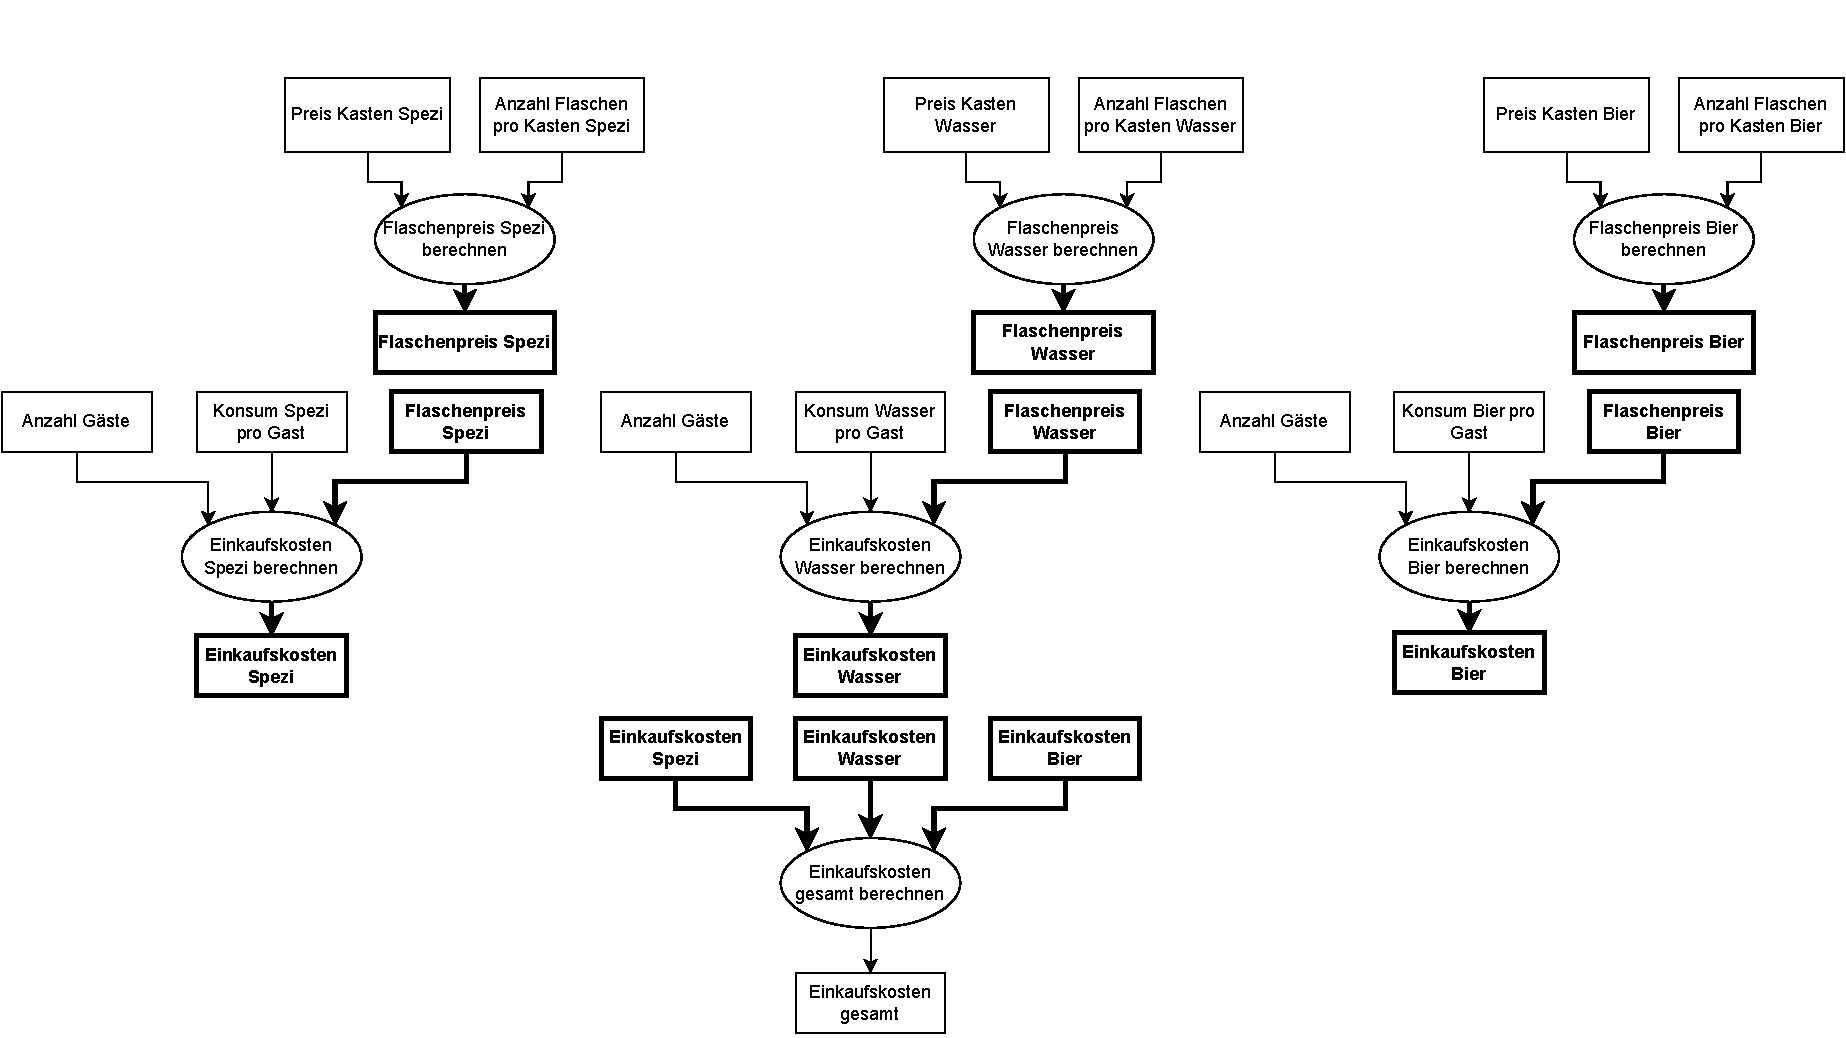
\includegraphics[width=\textwidth]{_Aufgaben/img/A06_Lsg_A01.pdf}
        }
        \definesframe[false]{}{
            \centering
            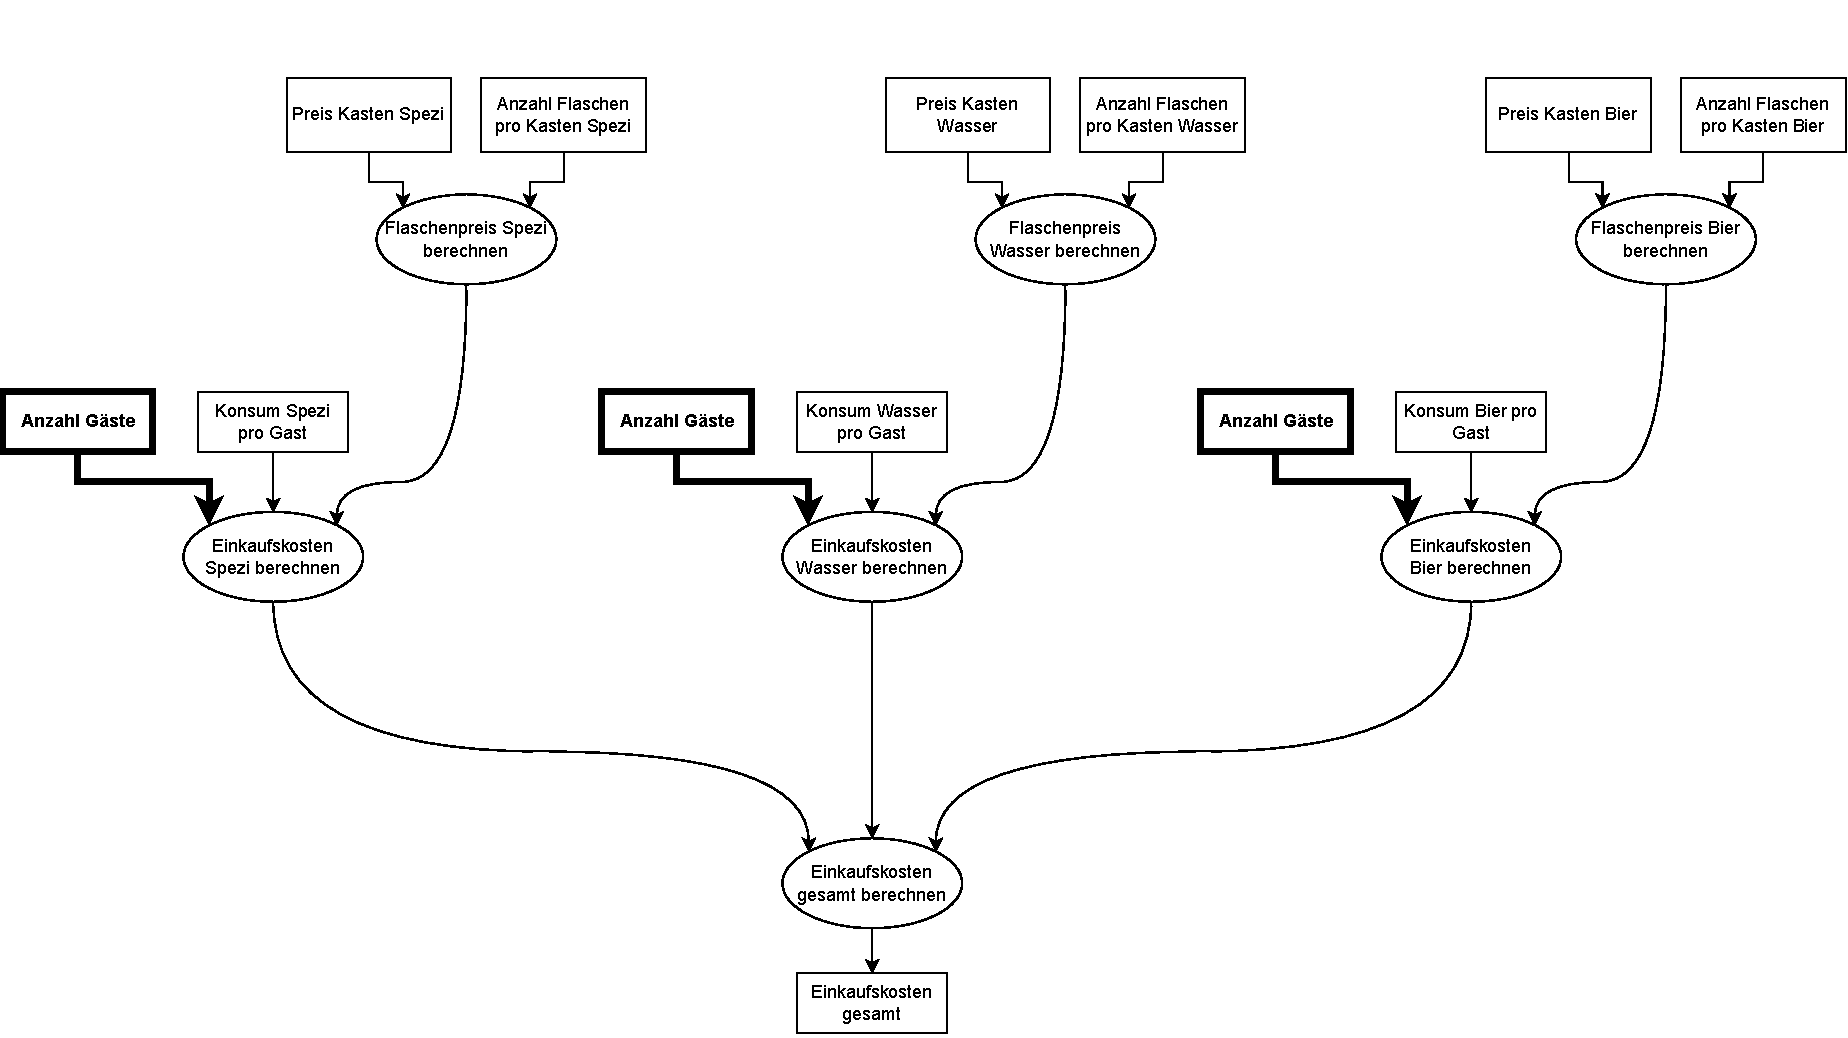
\includegraphics[width=\textwidth]{_Aufgaben/img/A06_Lsg_A02.pdf}
        }
        \definesframe[false]{}{
            \centering
            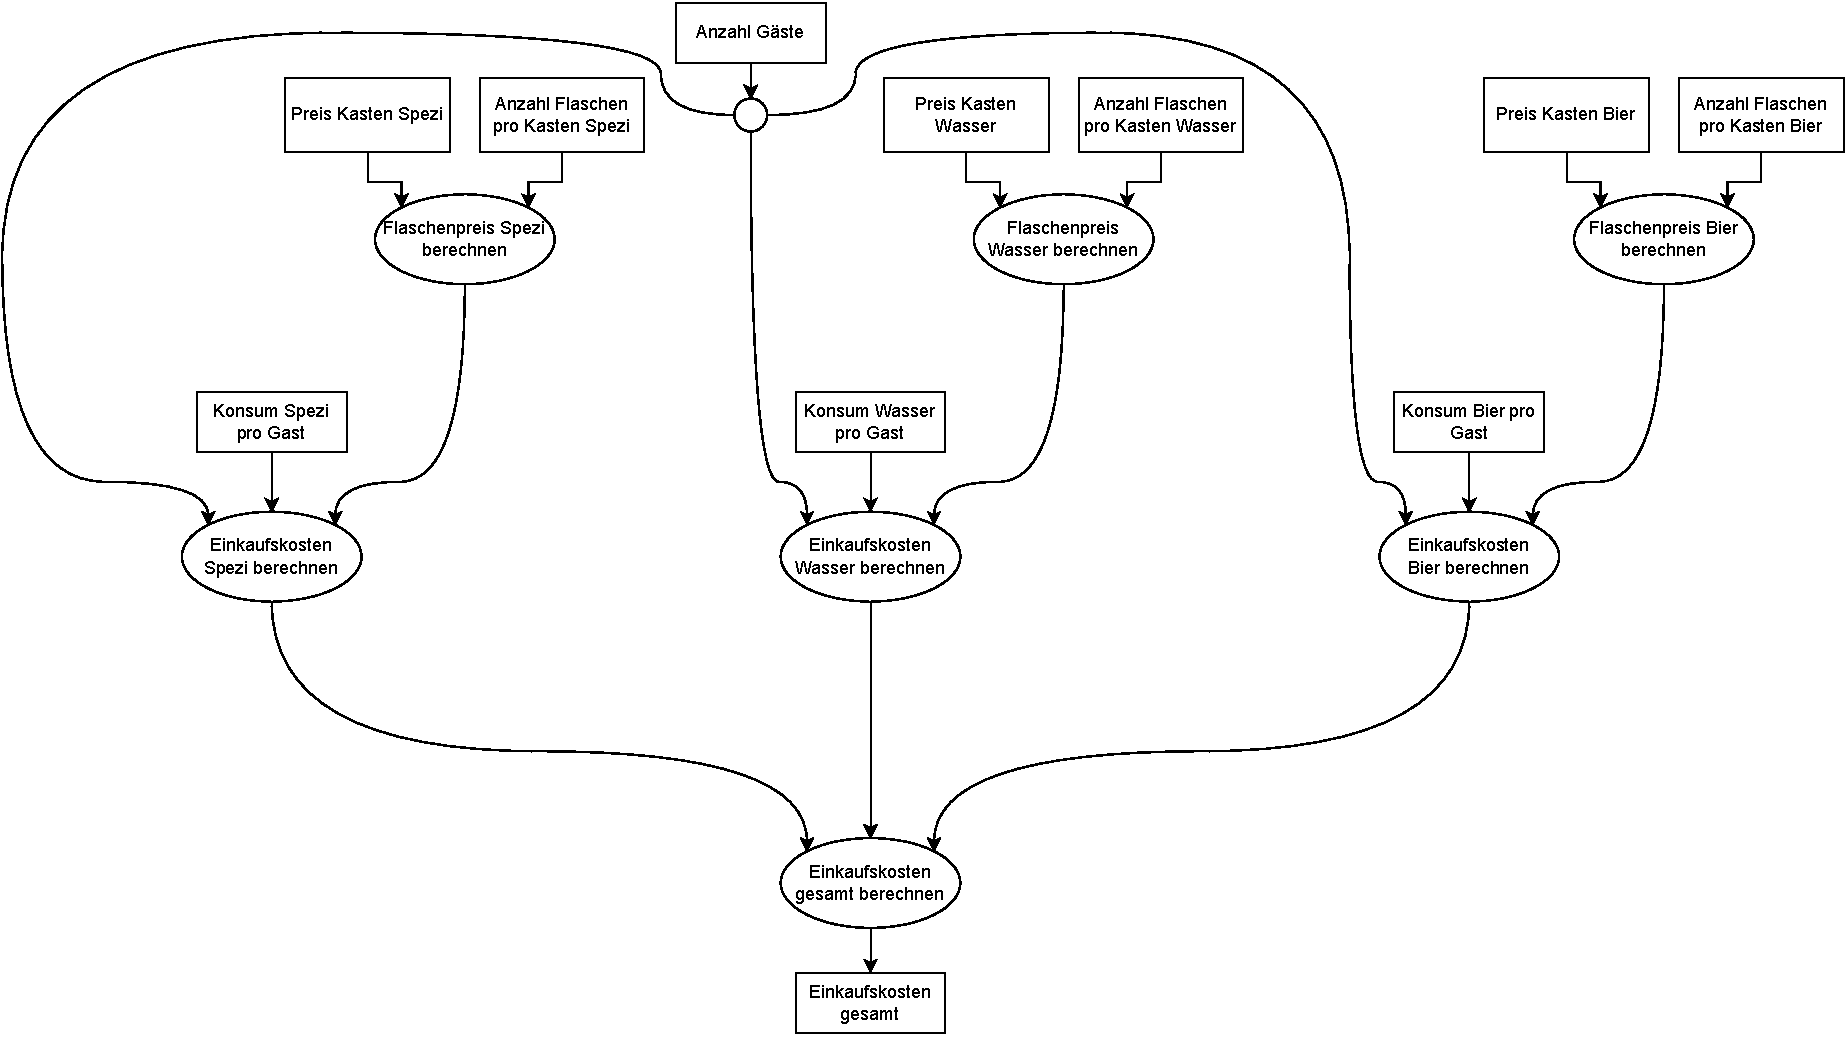
\includegraphics[width=\textwidth]{_Aufgaben/img/A06_Lsg_A03.pdf}
        }
    \else
        \UnterAufgabe{Gruppe A vereinfacht}{
            \Loesung{Gruppe A vereinfacht}
            
            \Loesung{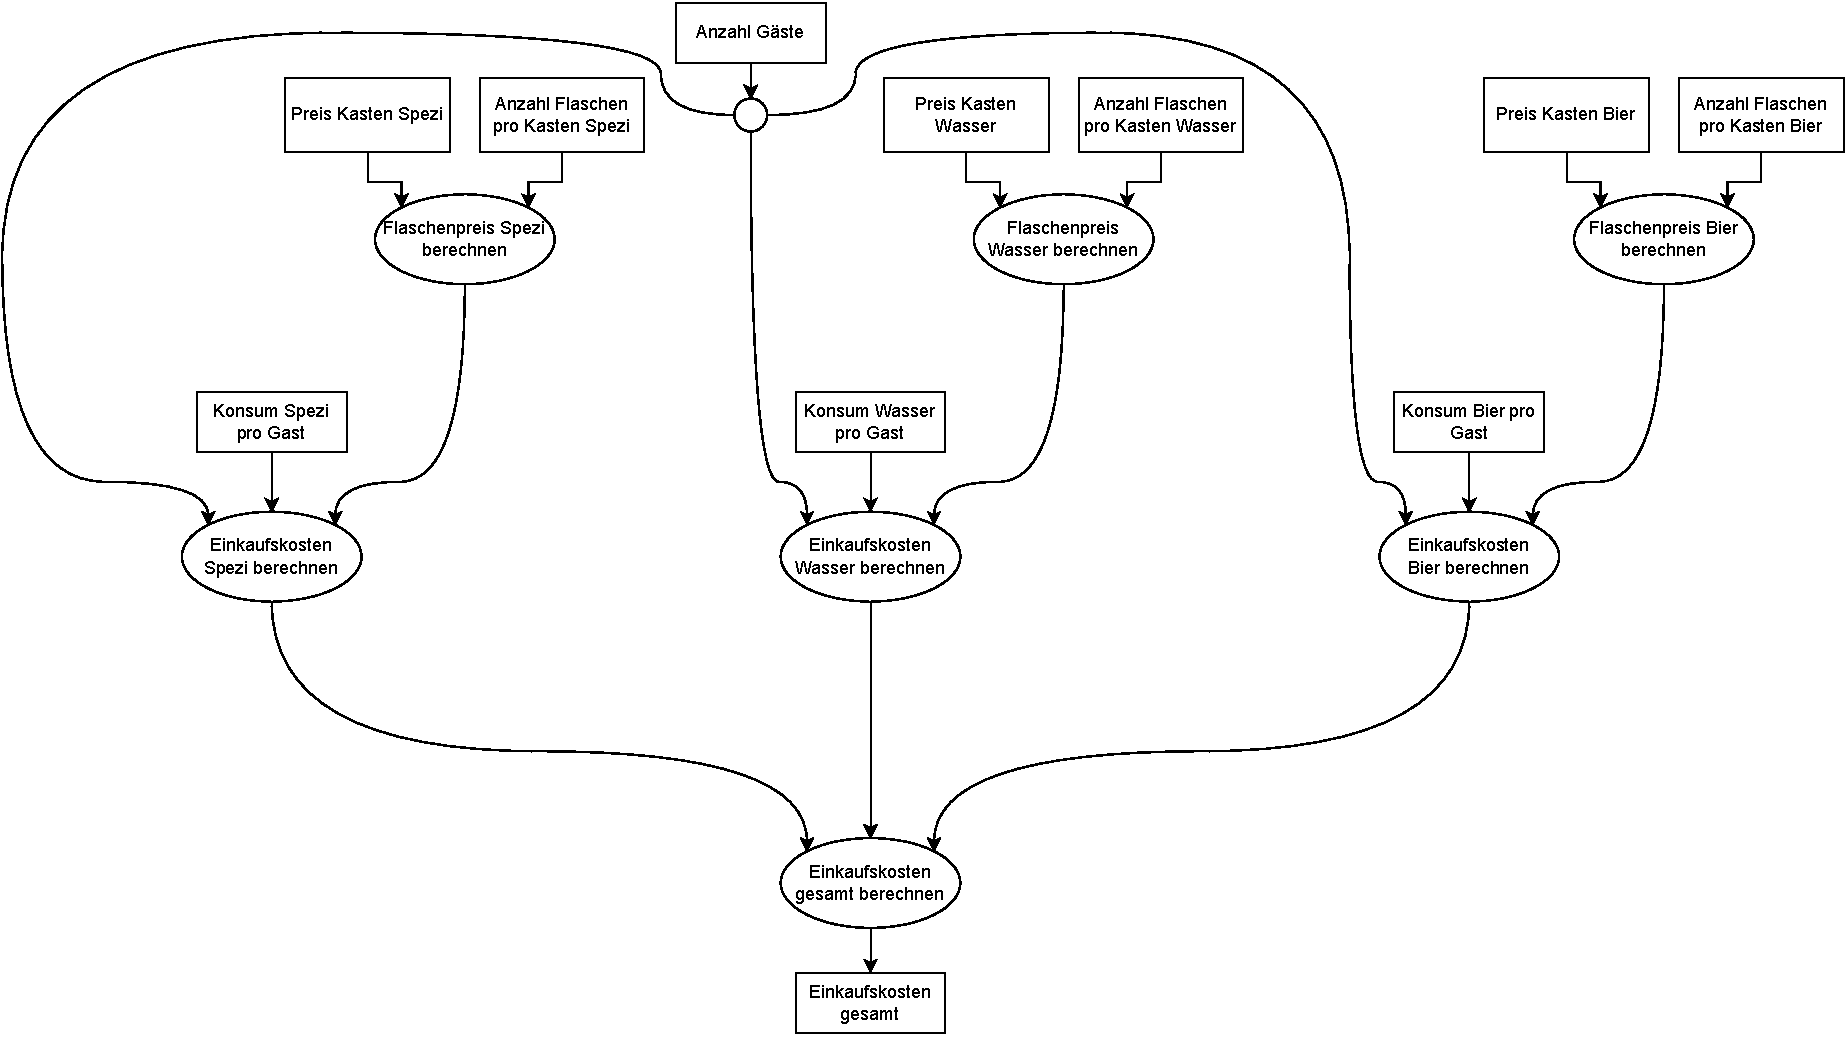
\includegraphics[width=\textwidth]{_Aufgaben/img/A06_Lsg_A03.pdf}}
        }
    \fi

    \ifbeamer
        \definesframe[false]{}{
            \centering
            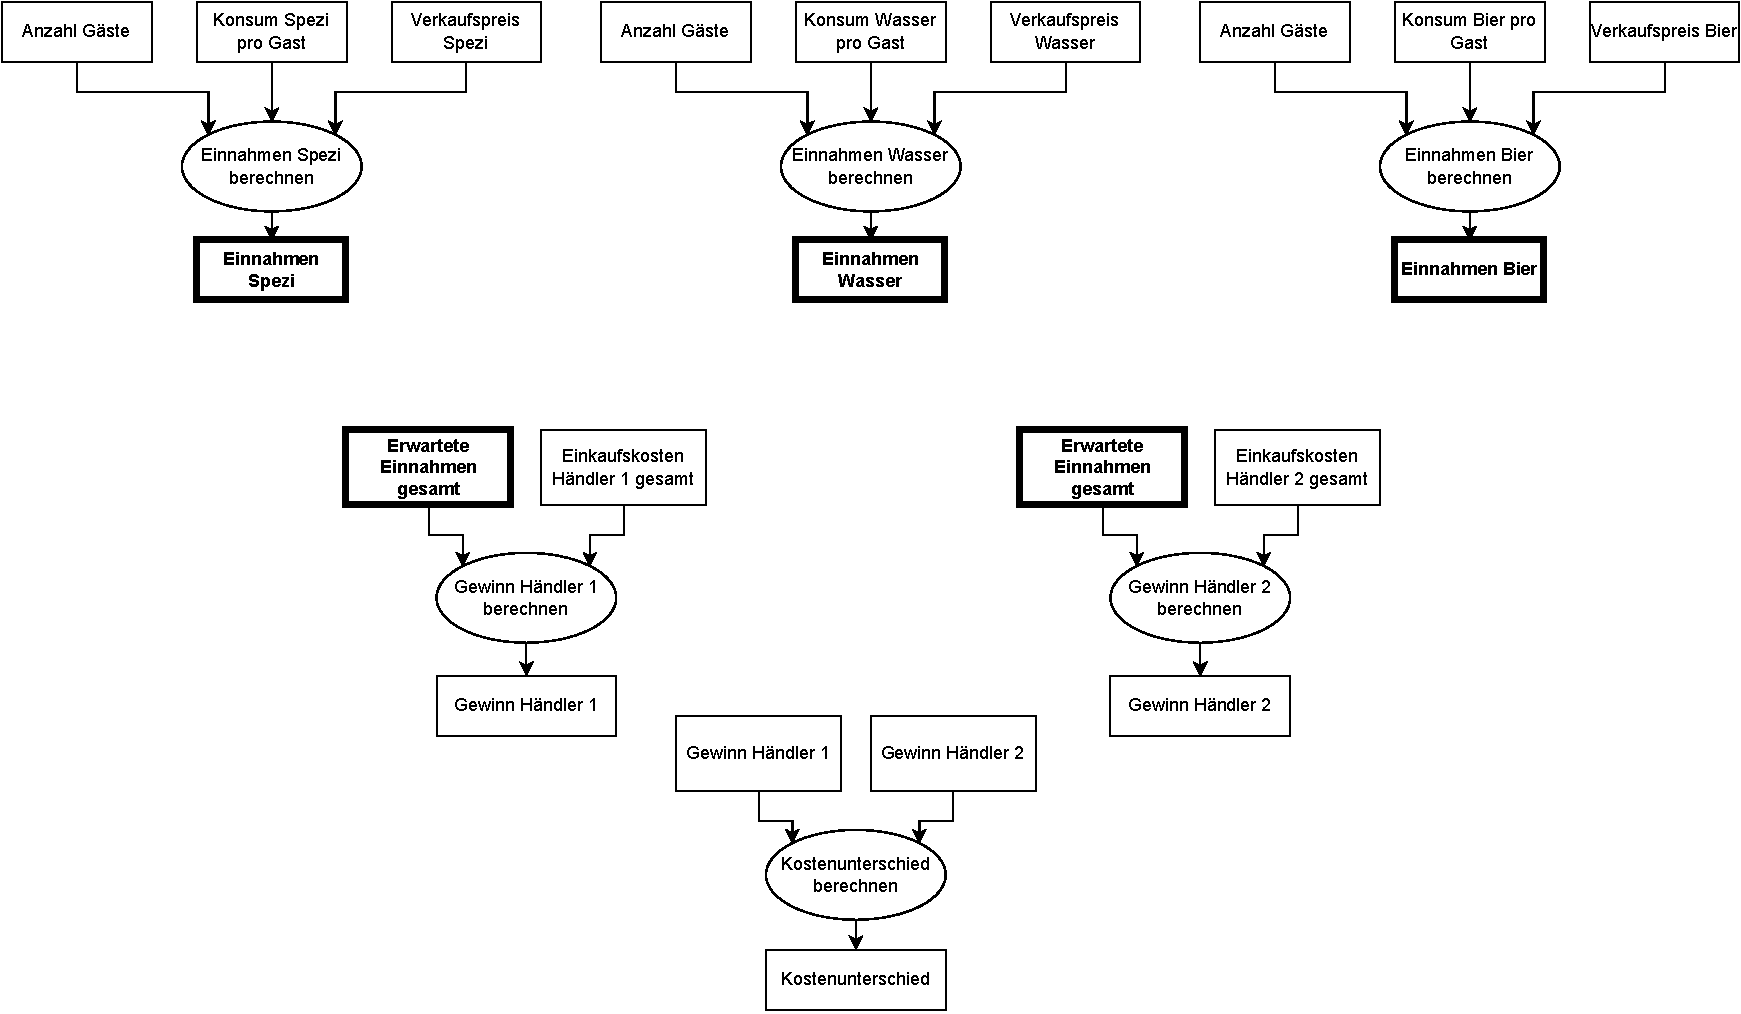
\includegraphics[height=\pageheight]{_Aufgaben/img/A06_Lsg_B01.pdf}
        }
        \definesframe[false]{}{
            \centering
            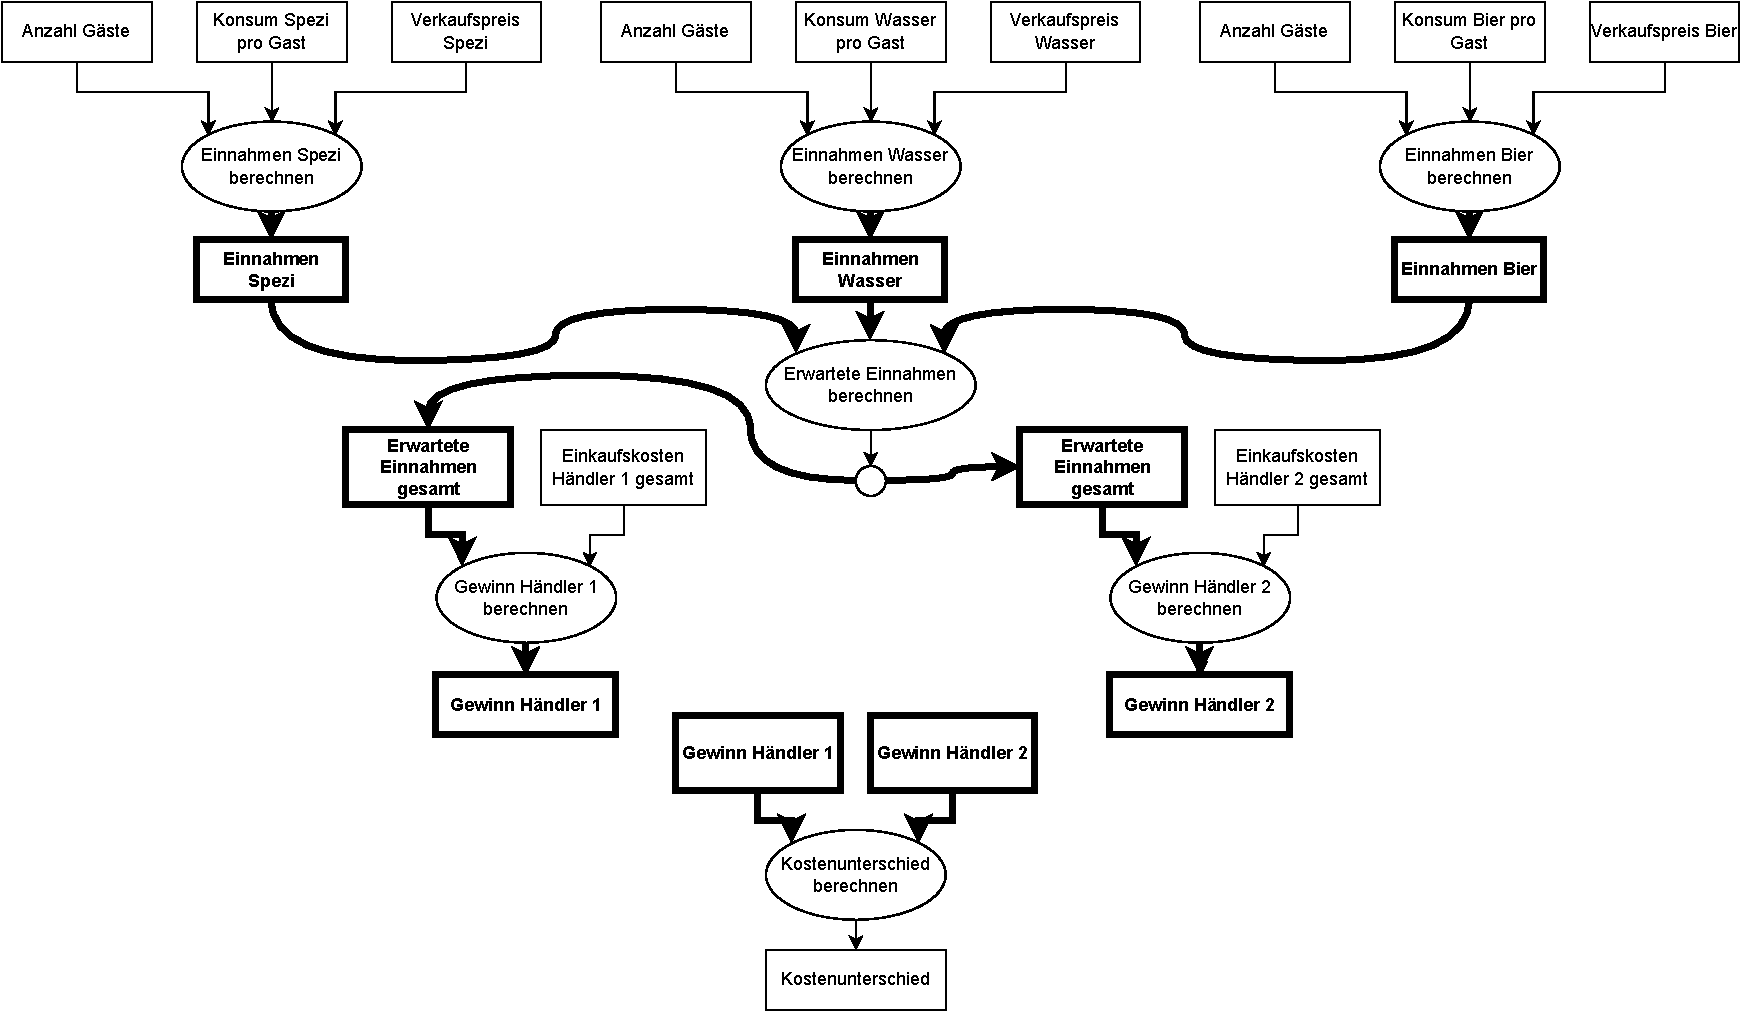
\includegraphics[height=\pageheight]{_Aufgaben/img/A06_Lsg_B02.pdf}
        }
        \definesframe[false]{}{
            \centering
            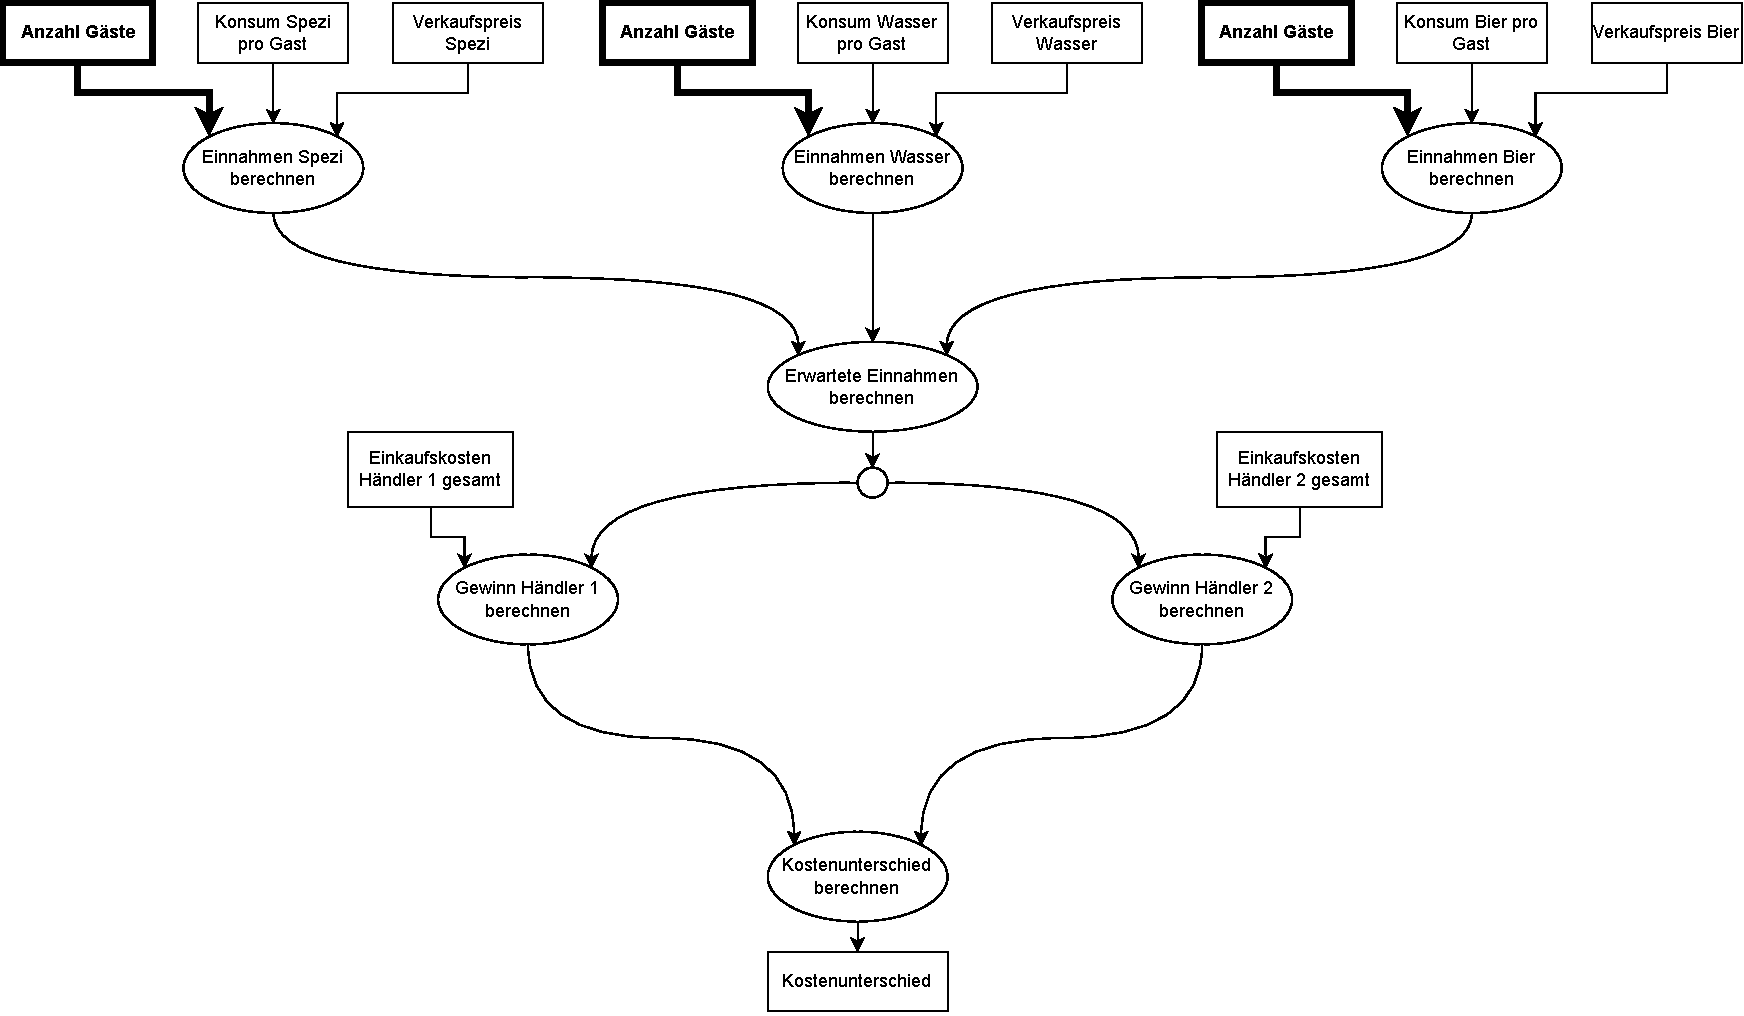
\includegraphics[height=\pageheight]{_Aufgaben/img/A06_Lsg_B03.pdf}
        }
        \definesframe[false]{}{
            \centering
            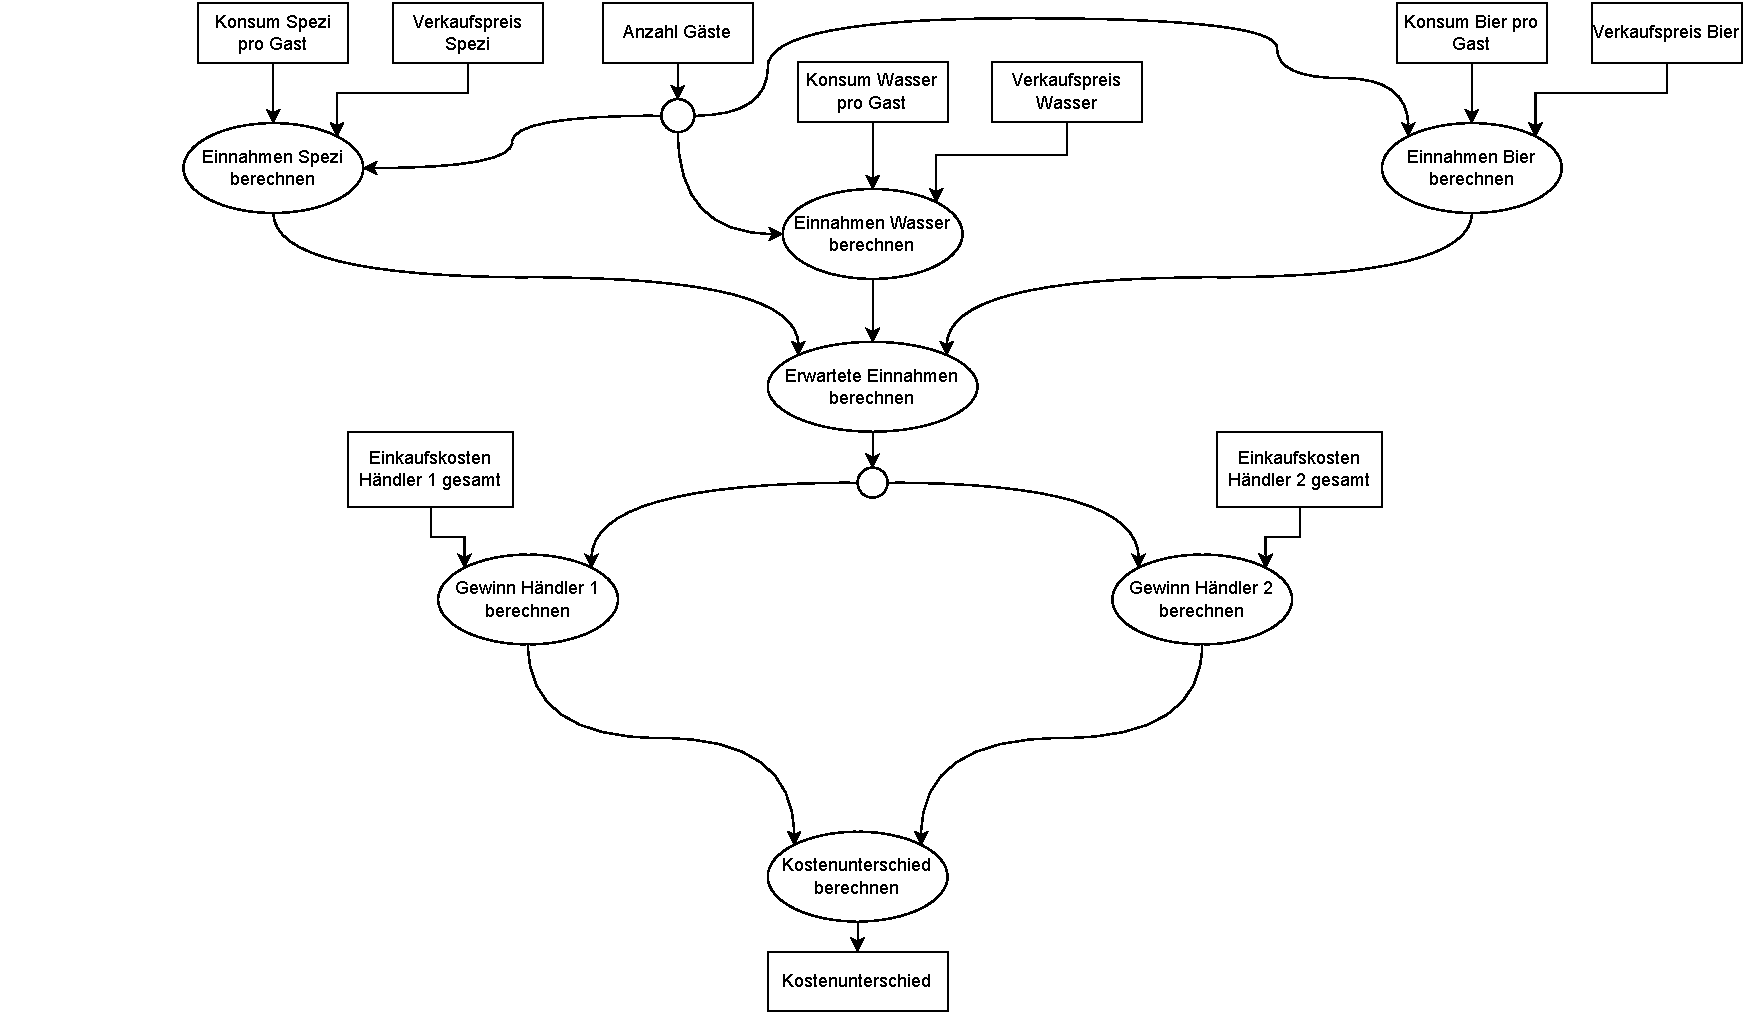
\includegraphics[height=\pageheight]{_Aufgaben/img/A06_Lsg_B04.pdf}
        }
    \else
        \UnterAufgabe{Gruppe B vereinfacht}{
            \Loesung{Gruppe B vereinfacht}
            
            \LoesungKaro{
                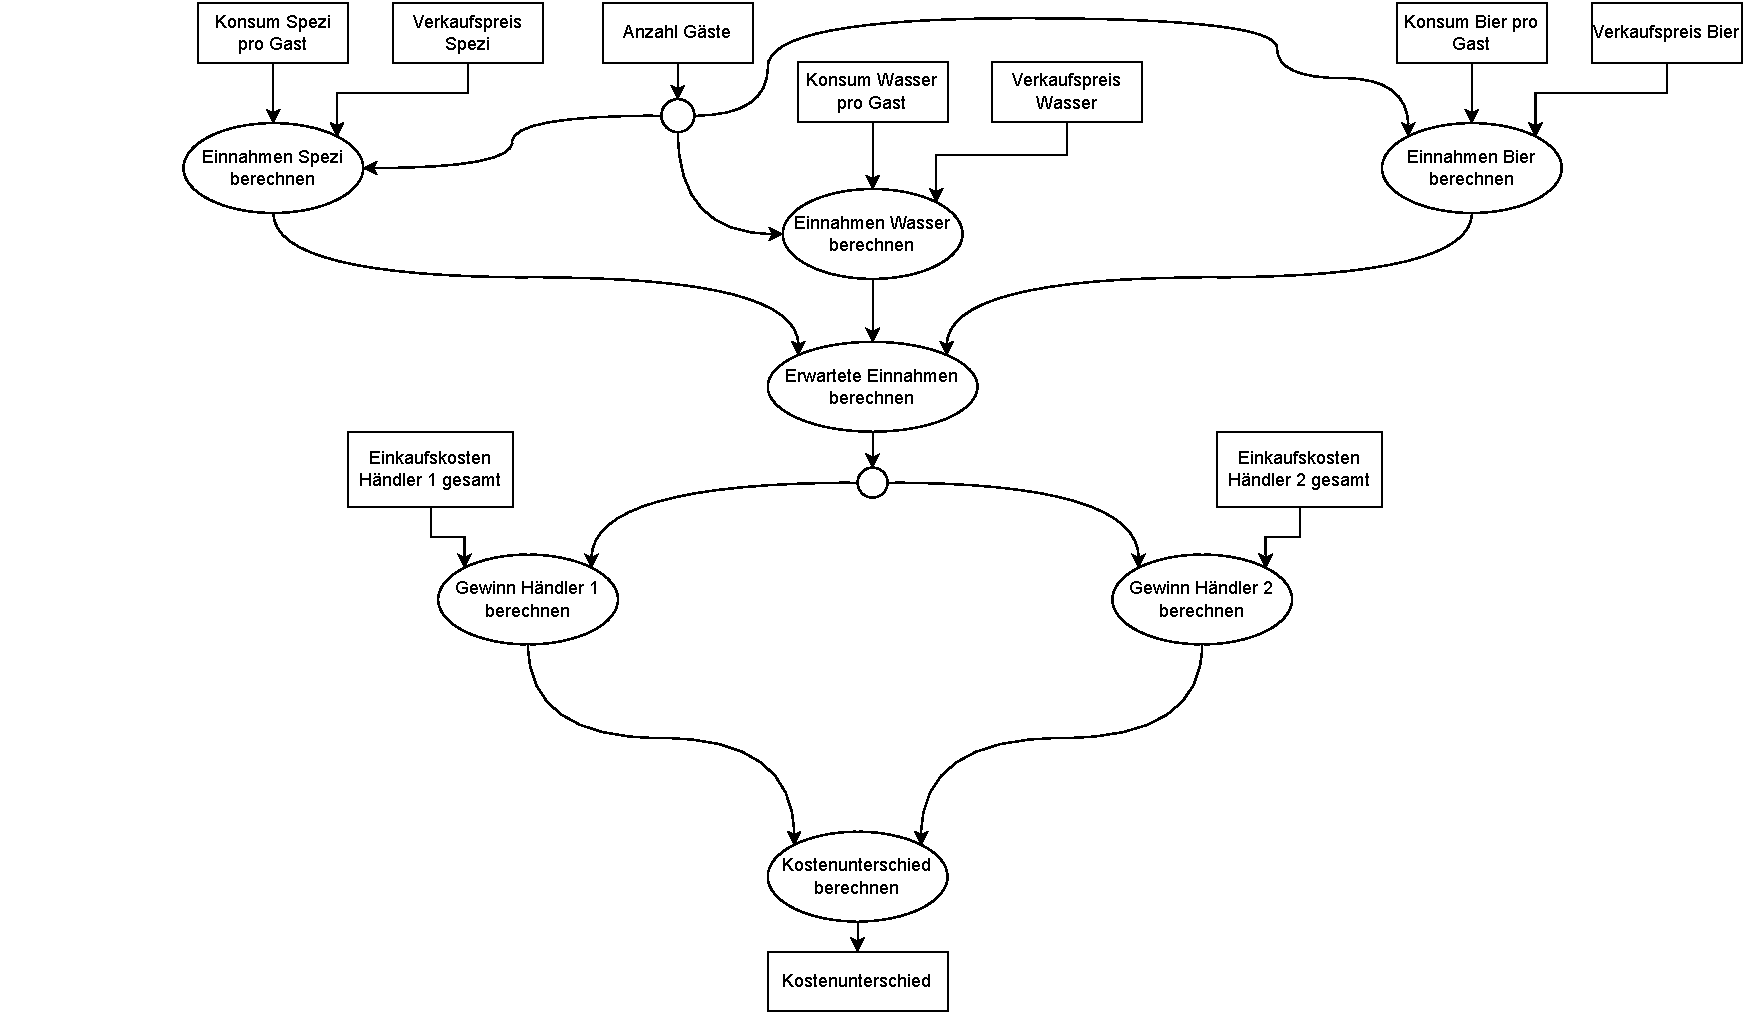
\includegraphics[width=\textwidth]{_Aufgaben/img/A06_Lsg_B04.pdf}
            }{51}
        }
    \fi
        
        \Hefteintrag{2}{Verkettung von Funktionen}{
    Wenn der \LoesungLuecke{Ausgabewert}{6cm} einer Funktion als \LoesungLuecke{Eingabewert}{6cm} einer anderen Funktion verwendet wird, spricht man von \LoesungLuecke{Verkettung}{6cm} von Funktionen. In Datenflussdiagrammen können \LoesungLuecke{Datenblöcke}{7cm} zwischen \LoesungLuecke{2 Funktionen}{10cm} weggelassen werden. Hierbei ist es dann besonders wichtig, aussagekräftige Funktionsnamen zu wählen. Mit einem \LoesungLuecke{Verteiler}{6cm} kann ein 

    \begin{minipage}[t]{0.5\textwidth}
        \vspace{-2cm}
        Datenfluss hierfür in zwei aufgeteilt werden:

        \vspace{12pt}
        Ein \emphColA{Beispiel} ist das Gesamt-Diagramm aus der  \emphColA{vorherigen Aufgabe}.
    \end{minipage}
    \hfill
    \begin{minipage}[t]{0.4\textwidth}
        \LoesungKaroTikz{
            \node[oval, minimum width=0.3cm, minimum height=0.3cm] (circ) {};
            \node[left=1cm of circ] (d1) {};
            \node[above right = 0.5cm and 1cm of circ] (d2) {};
            \node[below right = 0.5cm and 1cm of circ] (d3) {};

            \draw[arrow] (d1)--(circ);
            \draw[arrow] (circ)--(d2);
            \draw[arrow] (circ)--(d3);
        }{5}
        \vfill
    \end{minipage}
}
    }
    
    \mysession{Stunde 11+12}{
    
        \Aufgabe{Übung: Funktionale Modellierung}{
    Bei einer großen Party fallen nicht nur Getränkekosten an. Zeichne jeweils zwei Datenflussdiagramme: 
    \begin{itemize}
        \item Eines auf höchster Abstraktionsebene für Daten und Funktionen (genau eine Funktion pro Einzel-Diagramm).
        \item Eines mit konkreten Rechenoperationen in Funktionen (2-stellige Funktionen) und Daten auf höchster Abstraktionsebene.
    \end{itemize}
}
\UnterAufgabe{Übung: Funktionale Modellierung (a)}{
    
    \large\textbf{Getränkegewinn} \normalsize \hspace{0.2cm}
    Durch den Verkauf der Getränke nimmst du Geld ein. Am Ende der Party zählst du die Kassen und erhältst die Gesamteinnahmen. Aus diesem Betrag und den Ausgaben beim Lieferanten errechnest du den Gewinn.\\
    \doppelseite{0.5}{0.5}{t}{
        \LoesungKaroTikz{
            \node[dfddata, text width=2.2cm] (in) {Getränke Einnahmen};
            \node[dfddata, text width=2.2cm, right=1cm of in] (out) {Getränke Ausgaben};

            \node[oval, text width=4cm, below=1cm of $(in)!0.5!(out)$] (fkt) {Getränkegewinn berechnen};
            
            \node[dfddata, text width=4cm, below=0.7cm of fkt] (diff) {Getränke Gewinn};
            
            \draw[arrow] (in)--(fkt);
            \draw[arrow] (out)--(fkt);
                \draw[arrow] (fkt)--(diff);
        }{16}
    }{
        \LoesungKaroTikz{
            \node[dfddata, text width=2.2cm] (in) {Getränke Einnahmen};
            \node[dfddata, text width=2.2cm, right=1cm of in] (out) {Getränke Ausgaben};

            \node[oval, text width=4cm, below=1cm of $(in)!0.5!(out)$] (fkt) {-};
            
            \node[dfddata, text width=4cm, below=0.7cm of fkt] (diff) {Getränke Gewinn};
            
            \draw[arrow] (in)--(fkt);
            \draw[arrow] (out)--(fkt);
                \draw[arrow] (fkt)--(diff);
        }{16}
    }
}
\UnterAufgabe{Übung: Funktionale Modellierung (b)}{
    \begin{minipage}[t]{\textwidth}
    \large\textbf{Security} \normalsize \hspace{0.2cm}
    Weil die Feier deiner besten Freundin beim letzten Mal eskaliert ist, engagierst du einen Sicherheitsdienst. Die Anzahl der benötigten Security-Mitarbeiter berechnest du aus der Anzahl an Gästen und einem Personenschlüssel. Im Anschluss werden aus der Anzahl an Mitarbeitern und den Kosten pro Mitarbeiter die Security-Kosten berechnet.\\
    \doppelseite{0.5}{0.5}{t}{
        \LoesungKaroTikz{
            \node[dfddata, text width=2.2cm] (in) {Getränke Einnahmen};
            \node[dfddata, text width=2.2cm, right=1cm of in] (out) {Getränke Ausgaben};

            \node[oval, text width=4cm, below=1cm of $(in)!0.5!(out)$] (fkt) {Getränkegewinn berechnen};
            
            \node[dfddata, text width=4cm, below=0.7cm of fkt] (diff) {Getränke Gewinn};
            
            \draw[arrow] (in)--(fkt);
            \draw[arrow] (out)--(fkt);
                \draw[arrow] (fkt)--(diff);
        }{16}
    }{
        \LoesungKaroTikz{
            \node[dfddata, text width=2.2cm] (in) {Getränke Einnahmen};
            \node[dfddata, text width=2.2cm, right=1cm of in] (out) {Getränke Ausgaben};

            \node[oval, text width=4cm, below=1cm of $(in)!0.5!(out)$] (fkt) {-};
            
            \node[dfddata, text width=4cm, below=0.7cm of fkt] (diff) {Getränke Gewinn};
            
            \draw[arrow] (in)--(fkt);
            \draw[arrow] (out)--(fkt);
                \draw[arrow] (fkt)--(diff);
        }{16}
    }
    \end{minipage}
}

\UnterAufgabe{Übung: Funktionale Modellierung (c)}{
    \begin{minipage}[t]{\textwidth}
    \large\textbf{Anzahl Gäste} \normalsize \hspace{0.2cm}
    Du hast vergessen, am Einlass eine Strichliste zu führen, daher kennst du nur deine Einnahmen durch Eintrittskarten und wie viel eine gekostet hat. Hier raus berechnest du die Anzahl der Gäste.
    
    \LoesungKaro{}{13}
    
    \end{minipage}
}

\UnterAufgabe{Übung: Funktionale Modellierung (d)}{
    \begin{minipage}{\textwidth}
    \large\textbf{Gewinn pro Gast} \normalsize \hspace{0.2cm}
    Aus dem Getränke-Gewinn, den Security-Kosten und der Gästeanzahl berechnest du den durchschnittlichen Gewinn pro Gast.
    
    \LoesungKaro{}{15}
    \end{minipage}
}
    
\UnterAufgabe{Übung: Funktionale Modellierung (e)}{
    \begin{minipage}[t]{\textwidth}
    \large\textbf{Gesamt-Diagramm} \normalsize \hspace{0.2cm}
    Füge die vorherigen Einzel-Diagramme zu zwei verketteten Datenflussdiagrammen zusammen. 
    
    \LoesungKaro{}{45}
    \end{minipage}
}
        
        \Aufgabe{Umsetzung in Excel}{
\begin{enumerate}
    \item Setze die Diagramme aus der vorherigen Aufgabe in einer neuen Tabellendatei um.
    \item Überlege dir einen sinnvollen Aufbau für die Tabelle und hebe auch diesmal wieder den Typ (Eingabe, berechneter Wert, Beschriftung) der Zelle (z.B. farbig) hervor. 
    \item Achte darauf, dass auch die Zwischenergebnisse wie in den Datenflussdiagrammen in der Tabelle angezeigt werden.
\end{enumerate}  

Beschreibe deinen Ansatz grob:

\LoesungLine{
\begin{itemize}
    \item Möglichkeit 1: Einfach untereinander Eingaben und berechnete Werte etwa in Reihenfolge des 'Auftretens' 
    \item Möglichkeit 2: Strukturell am DFD orientiert, wird ähnlich einer Pyramide
    \item weitere Möglichkeiten: \dots
\end{itemize}

}{3}

Zeichne eine grobe Skizze deiner Tabelle:

\LoesungKaro{
    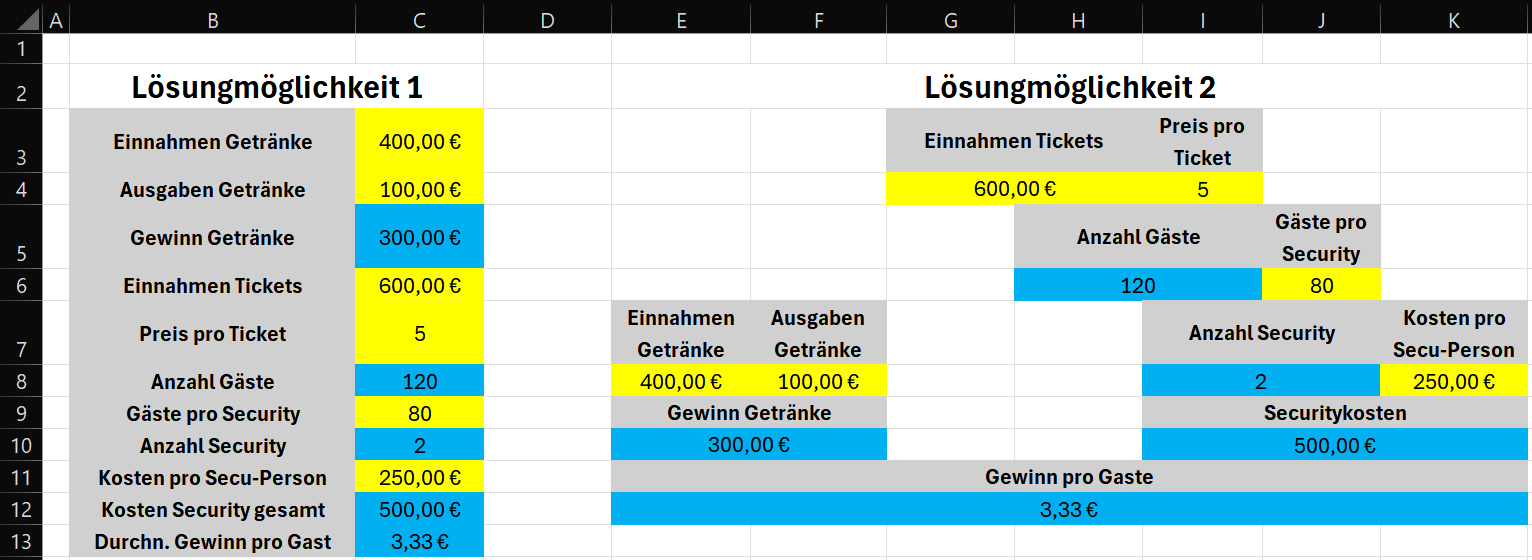
\includegraphics[width=\textwidth]{_Aufgaben/img/dfd_to_excel.png}
}{30}
}
    }
    
    \mysession{Stunde 13+14}{
        
        \Aufgabe[40]{Wenn-Dann-Funktion}{

%\vspace{0.5cm}
\begin{enumerate}
    \item Öffne Studyflix: \UrlAndCode{bycs.link/studyflix-excel-if}
    \item Schaue das Video und baue die beschriebene Tabelle in BYCS Drive nach.
    \item Fasse den Artikel/das Video in einem kurzen \emphColA{Hefteintrag} zusammen.
    \item Ergänze mit Hilfe deines Buchs, die Darstellung der Wenn-Dann-Funktion im Datenflussdiagramm.
\end{enumerate}

}
\Hefteintrag{1}{Wenn-Dann-Funktion}{
\ifbeamer\else\vspace{0.7cm}\fi
    \LoesungKaro{
        \doppelseite{0.55}{0.35}{t}{
            Mit der  \emphColA{Wenn-Dann-Funktion} können anhand einer Bedingung verschiedene Werte verwendet werden. 
            
            \vspace{0.2cm}
            Eine Bedingung kann z.B. 
            \begin{itemize}
                \item \emphColA{Gleichheit zweier Werte (=)} oder
                \item eine \emphColB{Größer-/Kleiner-Bedingung (<,>,<=,>=)}
            \end{itemize} 
            prüfen. 
            
            \vspace{0.1cm}
            Wenn die \emphColA{Bedingung} als \emphColA{wahr} ausgewertet \emphColA{(=erfüllt)} wird, wird der \emphColB{Dann-Teil in die Zelle eingefügt}, ansonsten der \emphColC{Sonst-Teil}.
            
            \vspace{0.1cm}
            In Excel gibt man die Funktion so ein:
            
            \vspace{0.2cm}
            Schema:~~~~=WENN(\emphColA{Bedingung}  ; \emphColB{Dann} ; \emphColC{Sonst})
            
            Beispiel:~~~~=WENN(\emphColA{D5 < 10} ; \emphColB{„kleiner als 10“} ; \emphColC{„größer oder gleich 10“})
        }{
            Bei der Darstellung im \emphColA{Datenflussdiagramm} ist die \emphColA{Reihenfolge} (von links nach rechts), mit der die \emphColA{Pfeile} an der Funktion ankommen, \emphColA{wichtig}:

            \vspace{0.2cm}
            \begin{tikzpicture}[
                % Define styles
                box/.style={rectangle, draw=\LFarbe, very thick, rounded corners, minimum width=3cm, minimum height=1cm,  text centered, text=\LFarbe, font=\large},
                oval/.style={ellipse, draw=\LFarbe, very thick, minimum width=3cm, minimum height=1.5cm, text centered, text=\LFarbe, font=\large},
                arrow/.style={-Stealth, thick, draw=\LFarbe},
                annotation/.style={text=colC!90!\LFarbe, font=\large}
            ]
            \node[dfddata, text width=1.8cm, minimum width=1pt] (e1) {Bedingung};
            \node[dfddata, text width=1.5cm, right=0.3cm of e1, minimum width=1pt] (e2) {Dann-Wert};
            \node[dfddata, text width=1.5cm, right=0.3cm of e2] (eN) {Sonst-Wert};
        
            \node[oval, text width=3cm, below=1cm of e2] (fkt) {WENN};
        
            \node[dfddata, below=0.75cm of fkt] (final) {Ausgabe};
            
            \draw[arrow] (e1) -- (fkt);
            \draw[arrow] (e2) -- (fkt);
            %\draw[arrow] (e3) -- (fkt);
            \draw[arrow] (eN) -- (fkt);
            \draw[arrow] (fkt) -- (final);
            \end{tikzpicture}
        }
    }{40}
}
        
        \Aufgabe[15]{Einkaufstabelle filtern}{
\AttachVlg{\faFileExcelO}{_Aufgaben/resources/A09_Vorlage.xlsx}
\begin{enumerate}
    \item Kopiert die freigegebene Einkaufstabelle in euren BYCS-Drive Ordner und Öffnet sie.
    \item Findet mit Hilfe der Filter Funktion folgendes heraus:\\
    \begin{itemize}
        \item Wie teuer war der teuerste Einkauf? \LoesungLuecke{649,90€}{4cm}\\
        \item Wie teuer war der teuerste Einkauf, den eine diverse Person mit Karte bezahlt hat? \LoesungLuecke{239,00€}{4cm}\\
        \item Wann und was war der erste Einkauf von Kosmetik in der Tabelle? \LoesungLuecke{14.01.2006, Haargummi}{4cm}\\
        \item Was ist der Name der alphabetisch ersten weibliche Person? \LoesungLuecke{Alicia Solis}{4cm}\\
        \item Was war der billigste Einkauf, der mit Karte gezahlt wurde? \LoesungLuecke{Milch}{4cm}
    \end{itemize}
\end{enumerate}
}

        
        \Hefteintrag{2}{Daten filtern}{
Verwaltet man große Datenmengen, ist es hilfreich, \emphColA{Filter} zu verwenden.
%
Mit diesen kann man:
\begin{itemize}
    \item nur \LoesungLuecke{Zeilen}{4cm} mit bestimmten Werten in einer \LoesungLuecke{Spalte}{4cm} anzeigen.
    \item die \LoesungLuecke{Zeilen}{4cm} nach den Werten einer bestimmten \LoesungLuecke{Spalte}{4cm} sortieren.
    \item Mehrere Filter können miteinander kombiniert werden.
\end{itemize}
}
    }

    \mysession{Zusatz}{
        \Aufgabe{Optional: Übung Notentabelle}{
Frau Knust möchte die Noten ihrer Klasse übersichtlich verwalten.

Hierfür benötigt sie eine Tabelle, in der die Gesamtnoten der einzelnen Fächer pro Schüler:in eingetragen werden, der Durchschnitt berechnet wird und in der letzten Spalte angezeigt wird, ob eine Person in mindestens zwei Fächern eine Note schlechter als 4 hat.

Die Notentabelle soll man mit der Filterfunktion sortieren und filtern können.
Die Tabelle soll außerdem optisch ansprechend sein.

Erstelle in BYCS-Drive eine solche Kalkulationstabelle
}
    }
}